    The subfigure package used to cause problems until James
    Gruetzner and Todd Pitts found out that the subfigure package
    uses {\tt addcontentsline}, which is redefined in the SANDreport
    class. The class uses the ifthen package, but it is not loaded
    at the time the subfigure package uses {\tt addcontentsline}.
    The new code avoids using the ifthen package.  Have a look at
    Figure~\ref{fig:creatures} for an example.

    \begin{figure}[!hbtp]
	\centering
	\subfigure[A Hyppogriff]{
	    \label{fig:sub:intro:creatures:hippogriff}
	    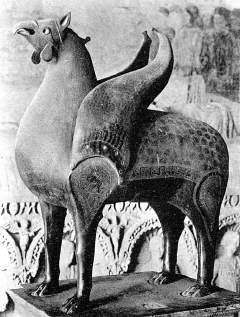
\includegraphics[keepaspectratio=true, width=2.0in]{hippogriff}
	}
	\subfigure[A Dragon]{
	    \label{fig:sub:intro:creatures:dragon}
	    
\includegraphics[keepaspectratio=true, width=2.0in]{dragon}
	}
	\caption{Creatures not drawn using dry-erase markers.}
	\label{fig:creatures}
    \end{figure}
